\documentclass{HW}

\newcommand{\hwtitle}{آزمایش پنج}
\newcommand{\studentname}{رادین شایانفر}
\newcommand{\studentnumber}{9731032}

\usepackage[top=30mm, bottom=30mm, left=25mm, right=25mm]{geometry}
\usepackage{amsthm,amssymb,amsmath,amsfonts}
\usepackage{fancyhdr}
\usepackage{changepage}
\usepackage{enumitem}
\usepackage{listings}
\usepackage[table]{xcolor}
\usepackage{fontspec}

\newfontfamily{\ttconsolas}{Consolas}

\definecolor{codegreen}{rgb}{0,0.6,0}
\definecolor{codegray}{rgb}{0.5,0.5,0.5}
\definecolor{codepurple}{rgb}{0.58,0,0.82}
\definecolor{backcolour}{rgb}{0.95,0.95,0.92}

\lstset{
  backgroundcolor=\color{backcolour},   
  commentstyle=\color{codegreen},
  keywordstyle=\color{magenta},
  numberstyle=\tiny\color{codegray},
  stringstyle=\color{codepurple},
  basicstyle=\ttconsolas\footnotesize,
  breakatwhitespace=false,         
  breaklines=true,                 
  captionpos=b,                    
  keepspaces=true,  
  numbers=left,                    
  numbersep=5pt,                  
  showspaces=false,                
  showstringspaces=false,
  showtabs=false,                  
  tabsize=4
}

\usepackage{array,multirow}

\usepackage{tikz}
\usetikzlibrary{trees}

% بسته‌‌ای برای ظاهر شدن شکل‌ها و تصاویر متن
\usepackage{graphicx}
\usepackage{color}
%بسته‌ای برای تنظیم فاصله عمودی خط‌های متن
\usepackage{setspace}

\usepackage[pagebackref=false,colorlinks,urlcolor=cyan,linkcolor=blue,citecolor=red]{hyperref}

\hypersetup{
    pdftitle={\hwtitle - \studentname - شماره دانشجویی: \studentnumber},
    bookmarks=true,
    pdfauthor={Radin Shayanfar},
}

% بسته‌ لازم برای تنظیم سربرگ‌ها
\usepackage{fancyhdr}

\usepackage{ptext} 
\usepackage{xepersian}

\doublespacing

\SepMark{-}
\settextfont[Scale=1.2]{B Nazanin}
\setlatintextfont{Times New Roman}
\renewcommand{\labelitemi}{$\bullet$}

\newcounter{mynumber}
\setcounter{mynumber}{1}
\newcommand{\mynum}{\arabic{mynumber}\stepcounter{mynumber}}

\newenvironment{question}{%
\medskip%
\par%
\noindent%
\textbf{سوال \mynum- \space}%
\smallskip
%\par\noindent\ignorespaces
\begin{adjustwidth}{7mm}{}
}{%
\end{adjustwidth}
\par\medskip
}

\fancypagestyle{first_page}{
\fancyhf{}
\fancyhead[C]{\raisebox{3ex}{\large \bfseries \hwtitle}}
\fancyhead[LO,LE]{\textbf{\studentname} \\
شماره دانشجویی: \studentnumber
\vspace{0.2mm}}
\fancyfoot[C]{\thepage{}}
\renewcommand{\headrulewidth}{1.2pt}
}

\fancypagestyle{pages}{
\fancyhf{}
\fancyhead[R]{\leftmark}
\fancyfoot[C]{\thepage{}}
\renewcommand{\headrulewidth}{1.2pt}
}

\begin{document}
\pagestyle{pages}
\thispagestyle{first_page}

\section{گام اول}

کد \lr{deviceQuery.cu} داده شده را کامپایل و اجرا می‌کنیم. مشخصات دستگاه را در شکل
\ref{fig:query}
مشاهده می‌کنیم.

\begin{figure}[ht!]
\begin{center}
	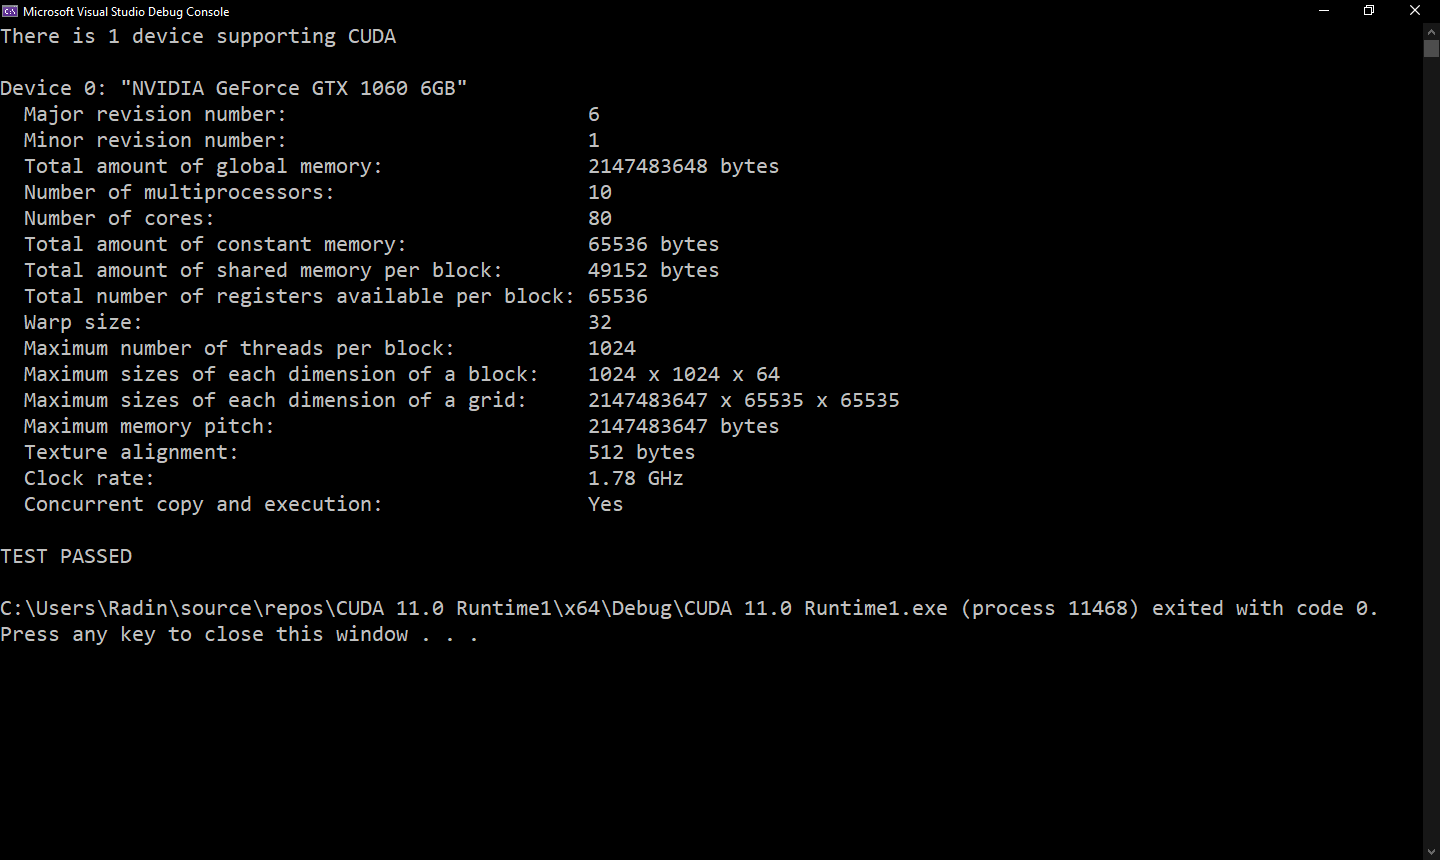
\includegraphics[width=15cm]{images/query}
\end{center}
\caption{مشخصات دستگاه با استفاده از کد \lr{deviceQuery}}
\label{fig:query}
\end{figure}

\section{گام دوم}

\begin{center}
\textbf{
زمان‌های اجرا میانگین ۱۰ بار اجرا است. همچنین زمان پر و کپی کردن بردارها و آزاد کردن حافظه در نظر گرفته نشده است.
}
\end{center}

برنامه جمع دو بردار را در حالت سریال بر روی \lr{CPU} اجرا می‌کنیم. زمان اجرا در حالت سریال به علت کوچک بودن برابر
\textbf{صفر}
 گزارش می‌شود.

با اضافه کردن تابع \lr{addWithCuda} و بردن محاسبات بر روی \lr{GPU} زمان اجرا به
\textbf{0/000048 ثانیه}
می‌رسد. دلیل کاهش سرعت اجرا، بالا بودن سربارهای بردن محاسبات روی \lr{GPU} نسبت به اندازه مسئله است.

\section{گام سوم}

به کد قسمت قبل متغیرهای
\lr{ELEMENTS\_PER\_THREAD}،
\lr{NUM\_THREADS}
و
\lr{NUM\_BLOCKS}
را اضافه می‌کنیم و تغییرات لازم را در کرنل انجام می‌دهیم. زمان‌های اجرای آزمایش شده در جدول
\ref{tab:gpuAdd}
آمده است (تسریع با میانگین‌گیری تسریع دو ستون انتهایی محاسبه شده است).

\begin{table}[ht]
\caption{زمان‌های اجرا (ثانیه) به ازای اندازه ورودی‌های مختلف}
\begin{center}
\begin{tabular}{|c|c|c|c|c|}
    \hline
    \multirow{2}{*}{موازی‌سازی} & \multicolumn{3}{|c|}{اندازه ورودی}& \multirow{2}{*}{تسریع} \\
    \cline{2-4}
& $2^{26}$ & $2^{27}$ & $2^{28}$ & \\
    \hline
  سریال & 
  0/071802 & 0/141790 & 0/281426 & - \\ \hline
  
  پردازش $n$ المان توسط هر نخ &
  0/153959 & 0/302569 & 1/038570 & 0/36 \\ \hline
  
  پردازش با $n$ بلوک & 
  0/005561 & 0/010990 & 0/021471 & 13/00 \\ \hline
\end{tabular}
\end{center}
\label{tab:gpuAdd}
\end{table}

در حالتی که هر نخ یک المان را پردازش می‌کند متغیر \lr{ELEMENTS\_PER\_THREAD} برابر یک قرار داده شده است. در حالت پردازش $n$ المان توسط هر نخ، مقدار این متغیر به شکل زیر محاسبه شده است.

\begin{latin}
%\begin{minipage}{\linewidth}
\begin{lstlisting}[language=C]
int ELEMENTS_PER_THREAD = size / 1024;
\end{lstlisting}
%\end{minipage}
\end{latin}

در شکل‌های
\ref{fig:gpu-coarse}
و
\ref{fig:gpu-fine}
به ترتیب خروجی برنامه در حالت پردازش $n$ المان توسط هر نخ و پردازش یک المان توسط $n$ بلوک برای اندازه ورودی $2^{28}$ آمده است.

 همانطور که می‌بینیم در حالت اول تنها یک بلوک نخ ۱۰۲۴ تایی داریم و هر نخ 262144 المان را پردازش می‌کند. این حالت به دلیل شباهت نحوه محاسبه به محاسبات روی \lr{CPU}، روی هسته‌های کوچک و ضعیف \lr{GPU} به خوبی جواب نمی‌دهد و اجرای آن \textbf{بسیار کندتر} است.
 
 در حالت دوم هر نخ تنها یک المان را پردازش می‌کند اما تعداد بلوک‌های ۱۰۲۴ تایی 262144 است. این کار (دادن کارهای کوچک به هر نخ و زیاد کردن تعداد نخ‌ها با افزایش تعداد بلوک‌ها) باعث استفاده حداکثری از قدرت \lr{GPU} می‌شود و زمان اجرا \textbf{به شدت کاهش} می‌یابد.
 
\begin{figure}[ht!]
\begin{center}
	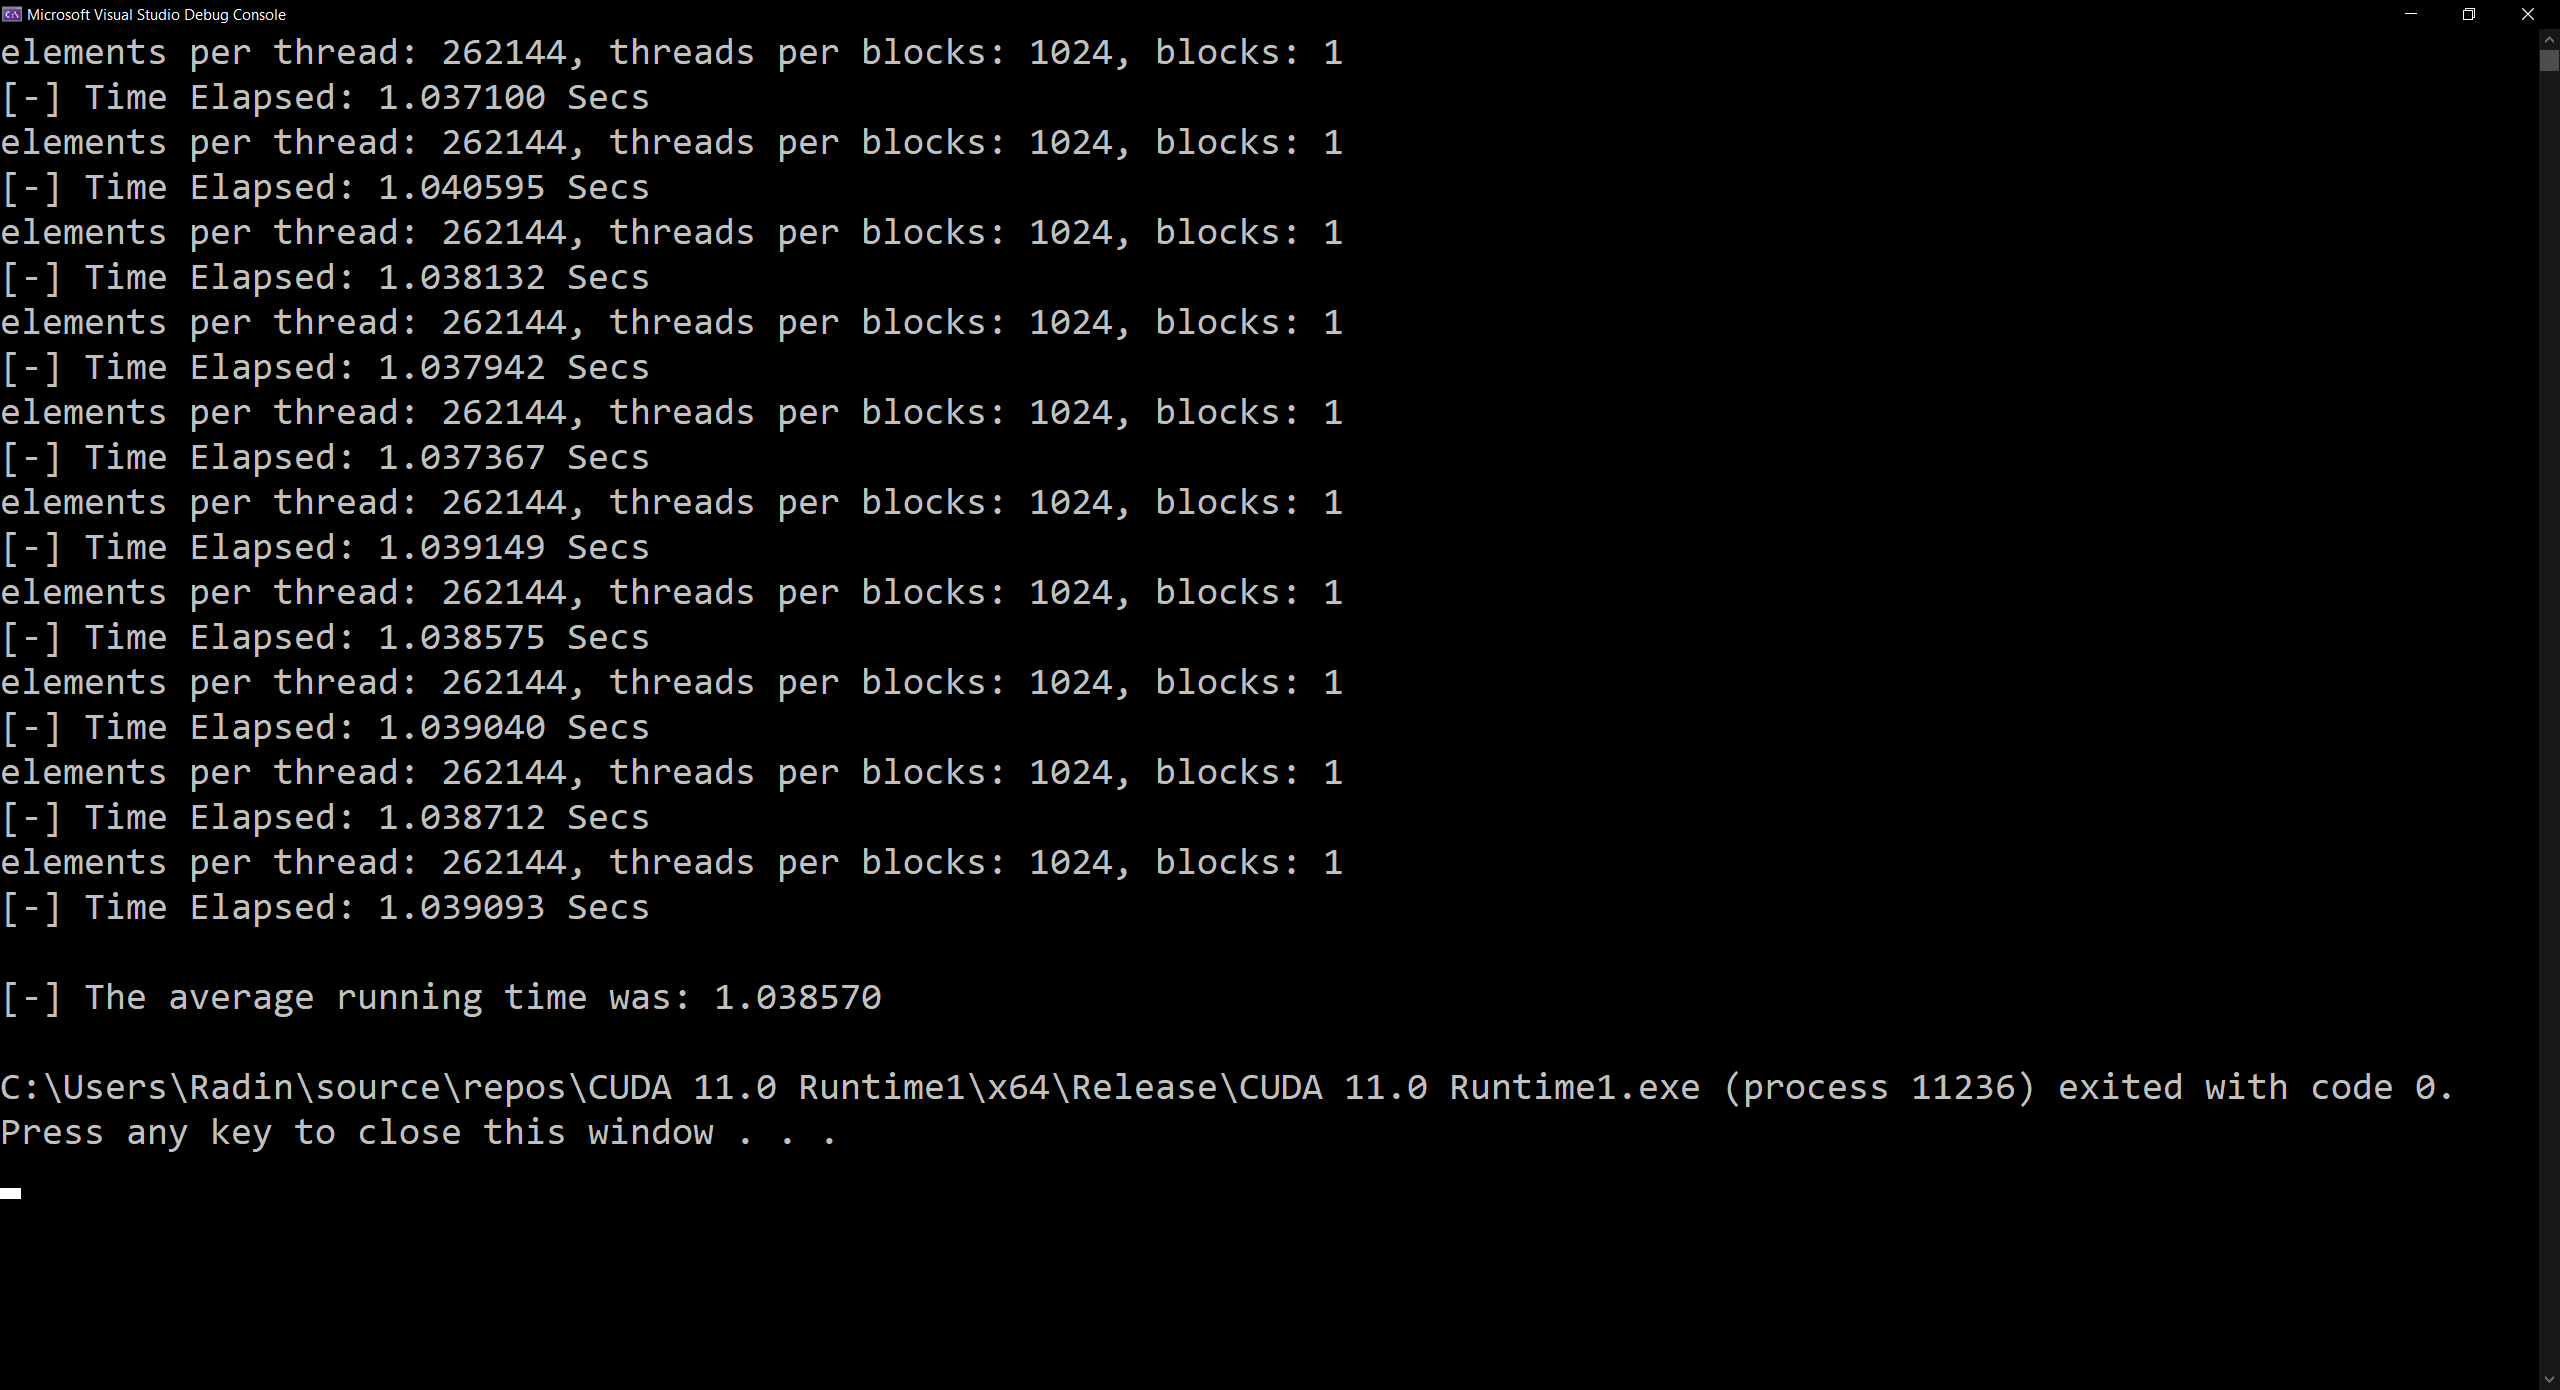
\includegraphics[width=15cm]{images/gpu-coarse}
\end{center}
\caption{پردازش
$n$
المان توسط هر نخ (درشت دانگی) منجر به کاهش شدید سرعت روی
\lr{GPU}
می‌شود.}
\label{fig:gpu-coarse}
\end{figure}

\begin{figure}[ht!]
\begin{center}
	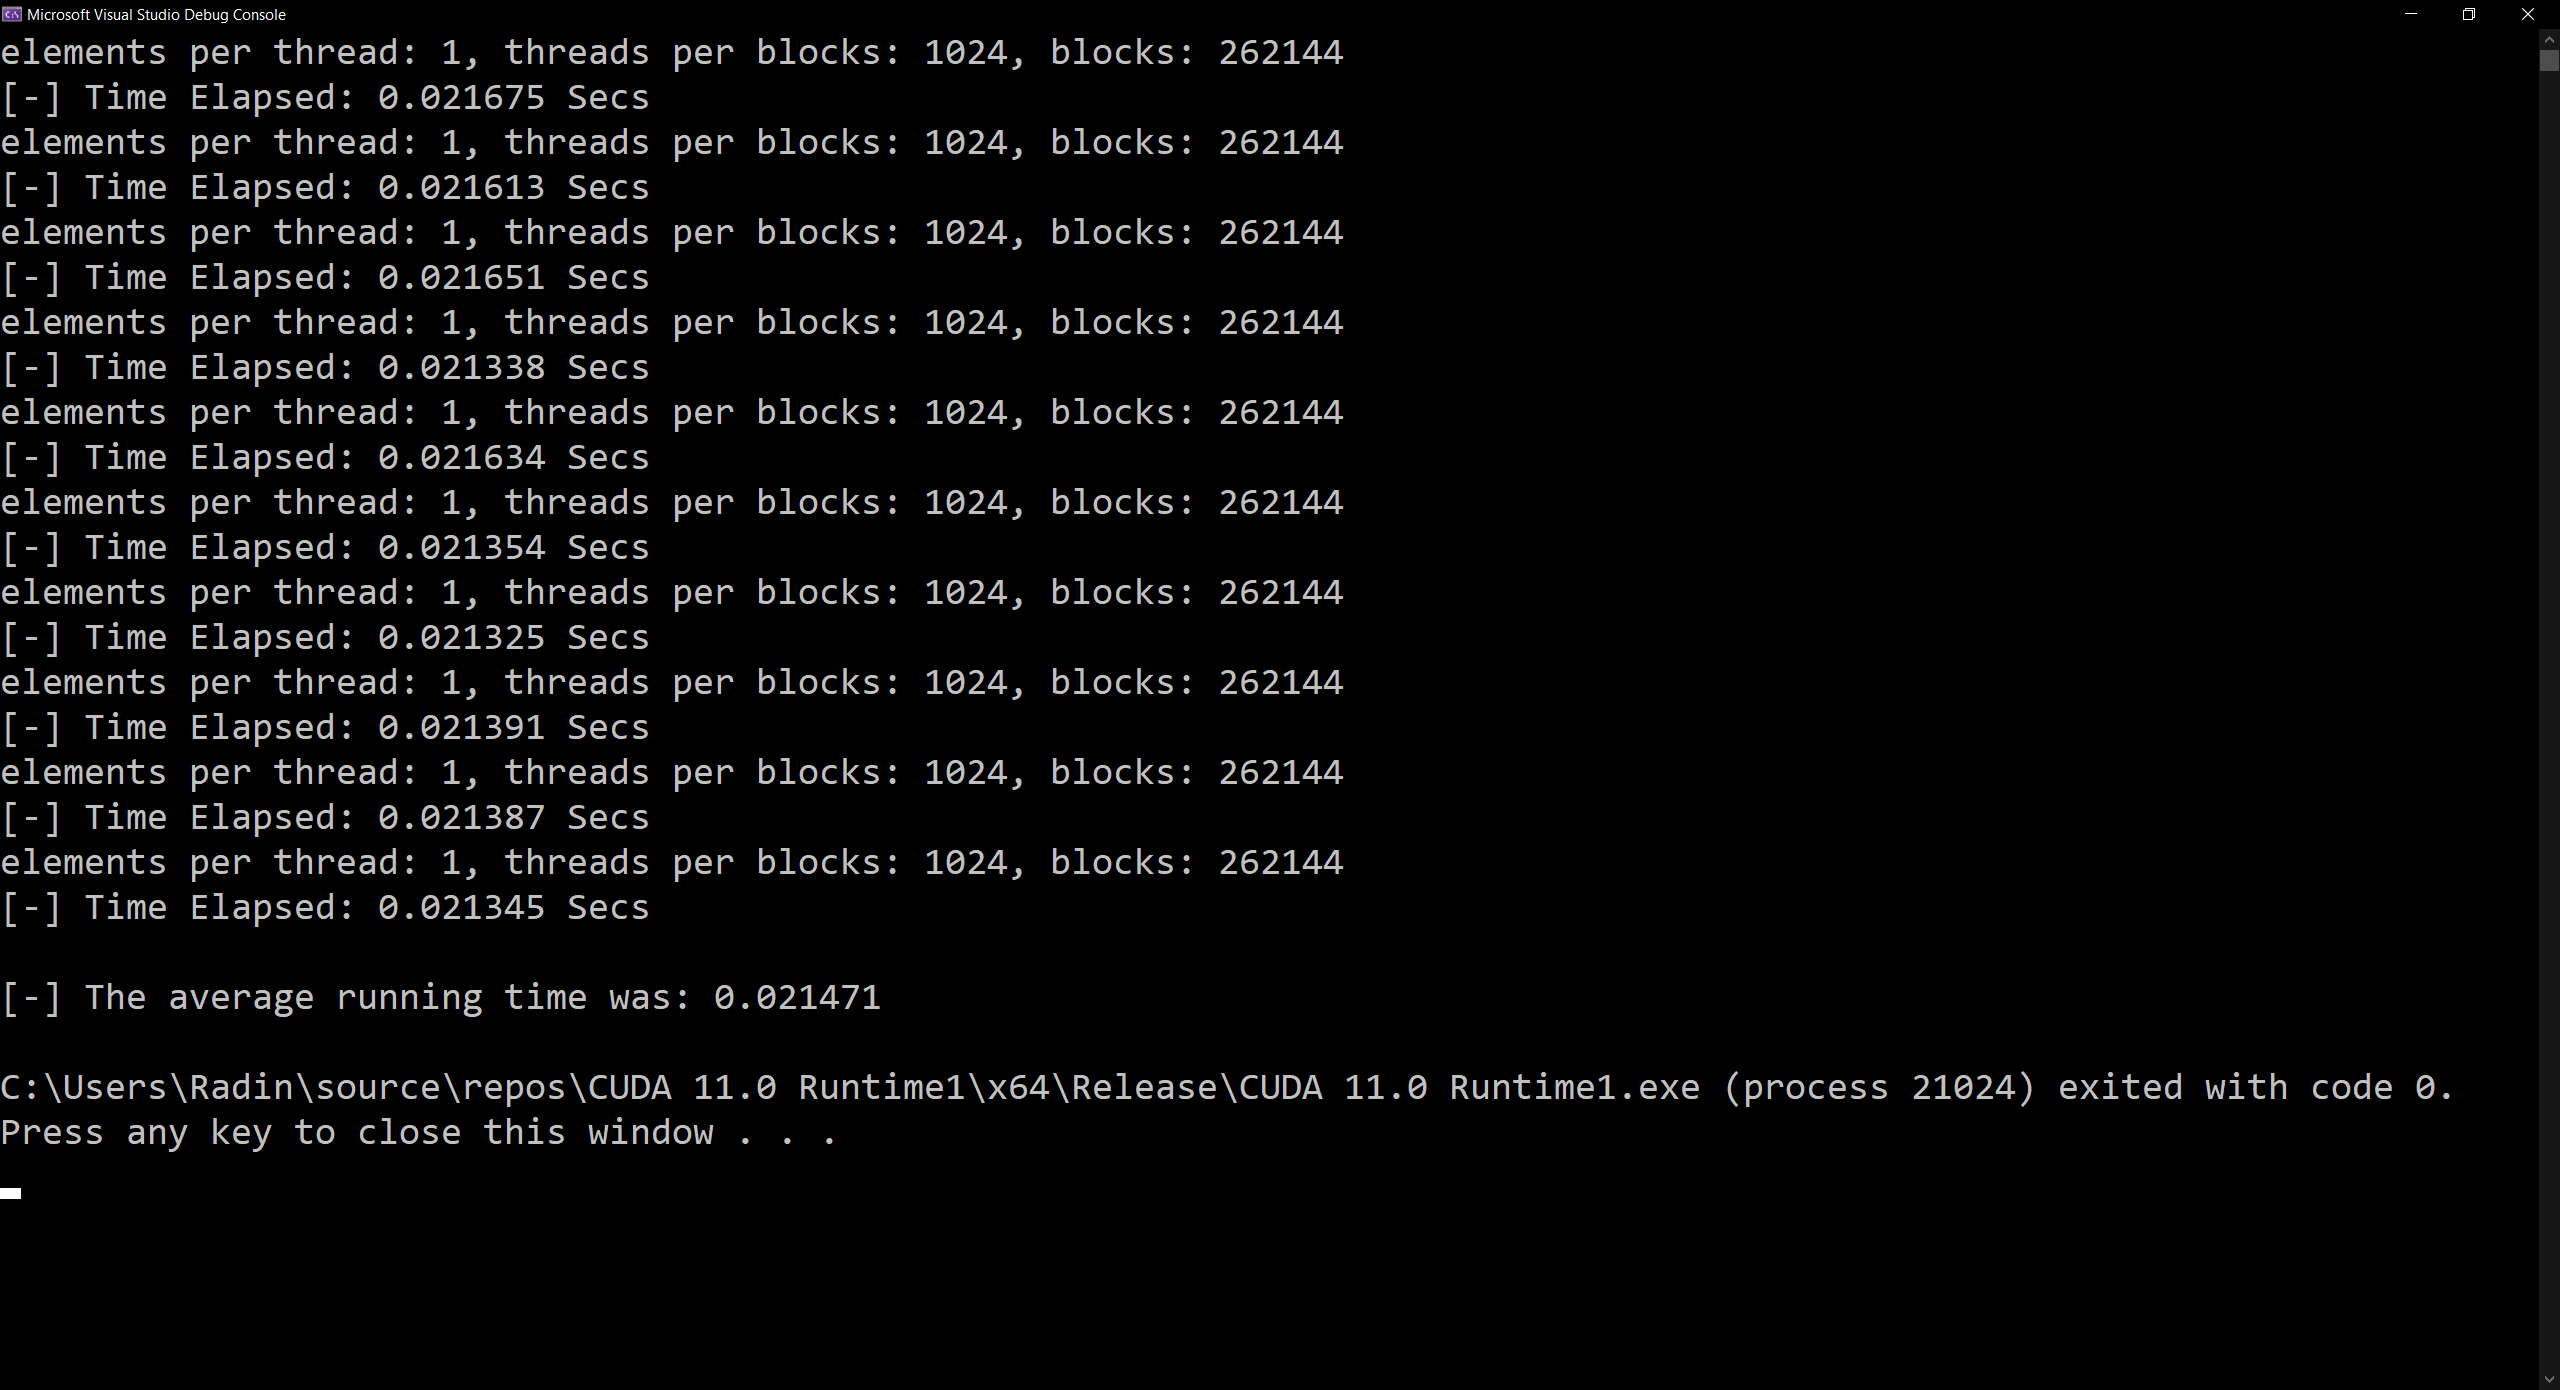
\includegraphics[width=15cm]{images/gpu-fine}
\end{center}
\caption{پردازش یک المان توسط هر نخ (ریز دانگی) منجر به کاهش شدید زمان اجرا و تسریع مناسب روی
\lr{GPU}
می‌شود.}
\label{fig:gpu-fine}
\end{figure}



\section{گام چهارم}

از آنجا که امکان استفاده از \lr{printf} در کرنل وجود ندارد، هر نخ موارد خواسته شده را داخل ۳ آرایه سراسری می نویسد. سپس در سمت \lr{host} این ۳ آرایه خوانده و چاپ می‌شوند. نمونه اجرای کد در شکل
\ref{fig:printf}
قابل مشاهده است (کد این بخش در فایل \lr{whoAmI.cu} قرار دارد).

\begin{figure}[ht!]
\begin{center}
	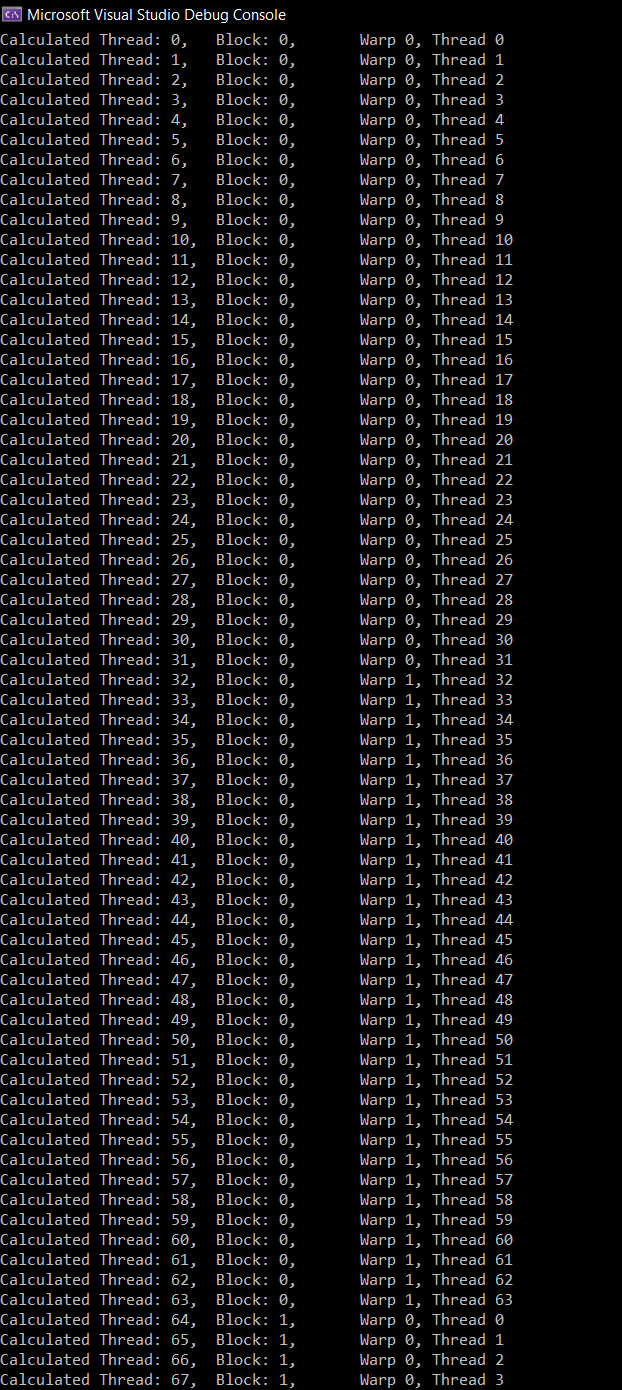
\includegraphics[height=17cm]{images/printf}
\end{center}
\caption{نحوه دسته‌بندی نخ‌ها داخل \lr{warp} و \lr{block}}
\label{fig:printf}
\end{figure}

\end{document}
